%% To submit your paper:
%DIF LATEXDIFF DIFFERENCE FILE
%DIF DEL archive/shumko_sampex_microburst_durations_v20.tex   Mon Jul 26 10:41:26 2021
%DIF ADD shumko_sampex_microburst_durations_v21.tex           Mon Aug  2 13:43:16 2021
\documentclass[draft]{agujournal2019}
\usepackage{url} %this package should fix any errors with URLs in refs.
\usepackage{lineno}
\usepackage[inline]{trackchanges}%for better trackchanges. finalnew option will compile document with changes incorporated.
\usepackage{soul}
\linenumbers
%%%%%%%
% As of 2018 we recommend use of the TrackChanges package to mark revisions.
% The trackchanges package adds five new LaTeX commands:
%
%  \note[editor]{The note}
%  \annote[editor]{Text to annotate}{The note}
%  \add[editor]{Text to add}
%  \remove[editor]{Text to remove}
%  \change[editor]{Text to remove}{Text to add}
%
% complete documentation is here: http://trackchanges.sourceforge.net/
%%%%%%%

\draftfalse

\journalname{Geophysical Research Letters}
%DIF PREAMBLE EXTENSION ADDED BY LATEXDIFF
%DIF UNDERLINE PREAMBLE %DIF PREAMBLE
\RequirePackage[normalem]{ulem} %DIF PREAMBLE
\RequirePackage{color}\definecolor{RED}{rgb}{1,0,0}\definecolor{BLUE}{rgb}{0,0,1} %DIF PREAMBLE
\providecommand{\DIFadd}[1]{{\protect\color{blue}\uwave{#1}}} %DIF PREAMBLE
\providecommand{\DIFdel}[1]{{\protect\color{red}\sout{#1}}}                      %DIF PREAMBLE
%DIF SAFE PREAMBLE %DIF PREAMBLE
\providecommand{\DIFaddbegin}{} %DIF PREAMBLE
\providecommand{\DIFaddend}{} %DIF PREAMBLE
\providecommand{\DIFdelbegin}{} %DIF PREAMBLE
\providecommand{\DIFdelend}{} %DIF PREAMBLE
%DIF FLOATSAFE PREAMBLE %DIF PREAMBLE
\providecommand{\DIFaddFL}[1]{\DIFadd{#1}} %DIF PREAMBLE
\providecommand{\DIFdelFL}[1]{\DIFdel{#1}} %DIF PREAMBLE
\providecommand{\DIFaddbeginFL}{} %DIF PREAMBLE
\providecommand{\DIFaddendFL}{} %DIF PREAMBLE
\providecommand{\DIFdelbeginFL}{} %DIF PREAMBLE
\providecommand{\DIFdelendFL}{} %DIF PREAMBLE
%DIF END PREAMBLE EXTENSION ADDED BY LATEXDIFF

\begin{document}

%% ------------------------------------------------------------------------ %%
%  Title
%
% (A title should be specific, informative, and brief. Use
% abbreviations only if they are defined in the abstract. Titles that
% start with general keywords then specific terms are optimized in
% searches)
%
%% ------------------------------------------------------------------------ %%



\title{Duration of Individual Relativistic Electron Microbursts: A Probe Into Their Scattering Mechanism}

\authors{M. Shumko\affil{1, 2}, L.W. Blum\affil{3}, and A.B. Crew\affil{4}}

\affiliation{1}{NASA's Goddard Space Flight Center, Greenbelt, Maryland, USA}
\affiliation{2}{Universities Space Research Association, Columbia, Maryland, USA}
\affiliation{3}{University of Colorado Boulder, Boulder, Colorado, USA}
\affiliation{4}{Johns Hopkins University Applied Physics Laboratory, Laurel, Maryland, USA}

\correspondingauthor{M. Shumko}{msshumko@gmail.com}

%% Keypoints, final entry on title page.

%  List up to three key points (at least one is required)
%  Key Points summarize the main points and conclusions of the article
%  Each must be 100 characters or less with no special characters or punctuation and must be complete sentences

\begin{keypoints}
\item We identified relativistic microbursts observed by the SAMPEX satellite and quantified their duration
\item The microburst duration interquartile range is 70-140 ms and shows trends in AE, L-shell, and MLT
\item In MLT, microburst durations double between midnight and noon---a trend similar to chorus element durations
\end{keypoints}

\begin{abstract}
We used the Solar Anomalous and Magnetospheric Particle Explorer (SAMPEX) to identify and quantify the duration of relativistic, $>1$ MeV, electron microbursts. A typical relativistic microburst has a $\approx 100$ millisecond (ms) duration, and the interquartile range of the duration distribution is 70-140 ms. We investigated trends in the microburst duration as a function of geomagnetic activity, L-shell, and magnetic local time (MLT). The clearest trend is in MLT: the median microburst duration doubles from \DIFdelbegin \DIFdel{80 }\DIFdelend \DIFaddbegin \DIFadd{75 }\DIFaddend milliseconds at midnight to \DIFdelbegin \DIFdel{160 }\DIFdelend \DIFaddbegin \DIFadd{140 }\DIFaddend milliseconds noon MLT. This trend is similar to the whistler mode chorus rising tone element duration trend, suggesting a possible relationship.
\end{abstract}

\section*{Plain Language Summary}
\noindent Energetic electron microbursts are an intense form of naturally occurring particle precipitation from the outer Van Allen Radiation Belt into Earth's atmosphere. Microbursts are observed in, or just above, the Earth's atmosphere, and are characterized by their short duration in time series data, often defined to be less than a second. The impact of microburst precipitation on the Earth's atmosphere is uncertain, but has been predicted to substantially degrade mesospheric ozone through the production of odd nitrogen and odd hydrogen molecules. Besides their environmental impact, we don't comprehensively understand how plasma waves, such as whistler mode chorus waves, scatter microbursts into our atmosphere. Therefore, in this study we quantified the duration of microbursts and used it as a proxy to understand how microbursts are scattered by these waves. We found that the microburst and chorus wave durations are correlated: their duration roughly doubles between the anti-sunward and sunward regions of the outer radiation belt.

\section{Introduction}\label{intro}
Earth's outer Van Allen radiation belt electron population is in constant flux, controlled by processes such as, radial transport, injections from the magnetotail, magnetopause shadowing, and local heating and loss into Earth's atmosphere due to wave-particle interactions \cite<e.g.>[and references within]{Ripoll2020}. Whistler mode chorus is one type of plasma wave, characterized by subsecond rising tone elements, that plays a dual role in electron dynamics: accelerate electrons from 10s of keV to MeV energies, and pitch angle scatter electrons into the atmosphere \cite<e.g.>{Li2009b, Thorne2010, Horne2003a, Summers2005}. One form of electron precipitation believed to be generated by chorus are microbursts: a subsecond intense increase of electrons. Microbursts were first observed by balloons in Earth's upper atmosphere, and later by satellites in low Earth orbit (LEO) \cite<e.g.>{Winckler1962, Anderson1964, Blake1996, Lorentzen2001a, O'Brien2003,Douma2017, Kurita2016}, and recently at high altitude near the magnetic equator \cite{Shumko2018b}.

Microburst electron energies span multiple orders of magnitude from tens of keV observed by, for example, \citeA{Datta1997}, to $>1$ MeV observed by the Solar Anomalous Magnetospheric Particle Explorer (SAMPEX) by \citeA{Blake1996}. Microbursts are predominately observed outside the plasmapause on the outer radiation belt footprints, $L\approx4-8$, and in the midnight to morning Magnetic Local Times (MLT) ($\approx 0-12$ hours MLT) \cite{Lorentzen2001a, Blum2015, O'Brien2003, Douma2017}. While microbursts are observed under all geomagnetic conditions, \citeA{Douma2017} showed that microburst occurrence frequency dramatically increases with the Auroral Electrojet (AE) index, and \citeA{O'Brien2003} showed a similar trend with the microburst frequency with the Disturbance storm time index phase.

The relative impact of energetic electron precipitation on the ionization of Earth's atmosphere and the depletion of radiation belt electrons is uncertain, but is estimated to be substantial. \citeA{Duderstadt2021} showed observations that suggest that electron precipitation can significantly impact atmospheric composition. The authors estimated a 20-30\% increase in atmospheric odd nitrogen ($\mathrm{NO_X}$), causing a 1\% decrease in ozone ($\mathrm{O_3}$)---substantial enough to affect the radiative balance in the upper atmosphere. Microbursts have also been estimated to be able to deplete the outer radiation belt electrons in hours to a few days, and models predict depletions of up to 20\% of upper mesospheric $\mathrm{O_3}$ \cite{O'Brien2004, Thorne2005, Douma2019,Breneman2017,Seppala2018}.

Electron microbursts are widely believed to be scattered by chorus waves. They were associated early on, due to the similar duration of microbursts and chorus rising tone elements and a similar occurrence distributions in MLT and L-shell \cite<e.g.>{Lorentzen2001a}. Furthermore, \citeA{Breneman2017} associated chorus rising tone elements to microbursts observed by the Focused Investigation of Relativistic Electron Bursts: Intensity, Range, and Dynamics CubeSats (FIREBIRD-II; \citeA{Crew2016, Johnson2020}) during a close magnetic conjunction.

A natural follow-on question is how are microbursts generated by chorus rising tone elements? For example, it is still unclear if relativistic ($>1$ MeV) microbursts are scattered via cyclotron resonance at high magnetic latitudes, or a higher resonance harmonic near the magnetic equator \cite{Lorentzen2001a}. One way to address this question is to study for how long microburst electrons are in resonance with a chorus wave. The resulting microburst duration, i.e. the microburst width in the time series data, is a probe into the conditions necessary to scatter microburst electrons. Thus, we used SAMPEX data to quantify the distribution of relativistic microburst durations as a function of L-shell, MLT, and the Auroral Electrojet index. We then compared these results to prior chorus rising tone element studies, and a chorus-electron test particle model. 

\section{Instrumentation}\label{instrumentation}
For this study we used the $>1$ MeV electron data, taken by the Heavy Ion Large Telescope (HILT) instrument \cite{Klecker1993} onboard the SAMPEX satellite \cite{Baker1993}. SAMPEX was launched in July 1992 and reentered Earth's atmosphere in November 2012. It was in a 520x670 km, $82^\circ$ inclination low Earth orbit. In general, SAMPEX had two pointing modes: spin and orbit rate rotation (zenith pointing). To avoid the compounding effects due to the variable pitch angles sampled in the spin mode, we only used the zenith pointing mode data. The International Geomagnetic Reference Field \cite[IGRF]{Thebault2015} magnetic field model was used to derive the geomagnetic coordinates.

The HILT instrument consisted of a large rectangular chamber with the aperture on one end, and 16 solid state detectors on the other. We used the HILT electron data taken between 1997 and 2012 (state4 in the data archive). The electron counts were accumulated from all of the solid state detectors at a 20 ms cadence.

\section{Methodology}\label{methodology}

\subsection{Microburst Identification}\label{microburst_id}
First, we identified microbursts using the burst parameter defined by \citeA{O'Brien2003}, also used in numerous other SAMPEX microburst studies \cite<e.g.>{Douma2017}. Assuming Poisson probability for the observed electron counts, the burst parameter is the number of standard deviations of a foreground signal above the background, expressed as
\begin{equation}
n_\sigma = \frac{N-A}{\sqrt{A+1}}
\end{equation} where $N$ is the number of foreground electron counts, and $A$ is the centered running average background counts. The $1$ in the denominator prevents a division by 0 error. In \citeA{O'Brien2003}, and in the results in this study, $N$ was summed over 100 ms and is called $N_{100}$, while $A$ was summed over 500 ms and is likewise called $A_{500}$.  Henceforth, we specify the time windows with subscripts for $N$ and $A$. Times when $n_\sigma > 10$ are classified as burst times, and the peak time in each continuous burst time interval is saved to the microburst data set. With $A_{500}$ and $N_{100}$, we detected a total of 256,764 microbursts over the 15 year period from 1997 to 2012. Four examples of microbursts are shown in Fig. \ref{fig1} by the solid black curves.

\begin{figure}
\noindent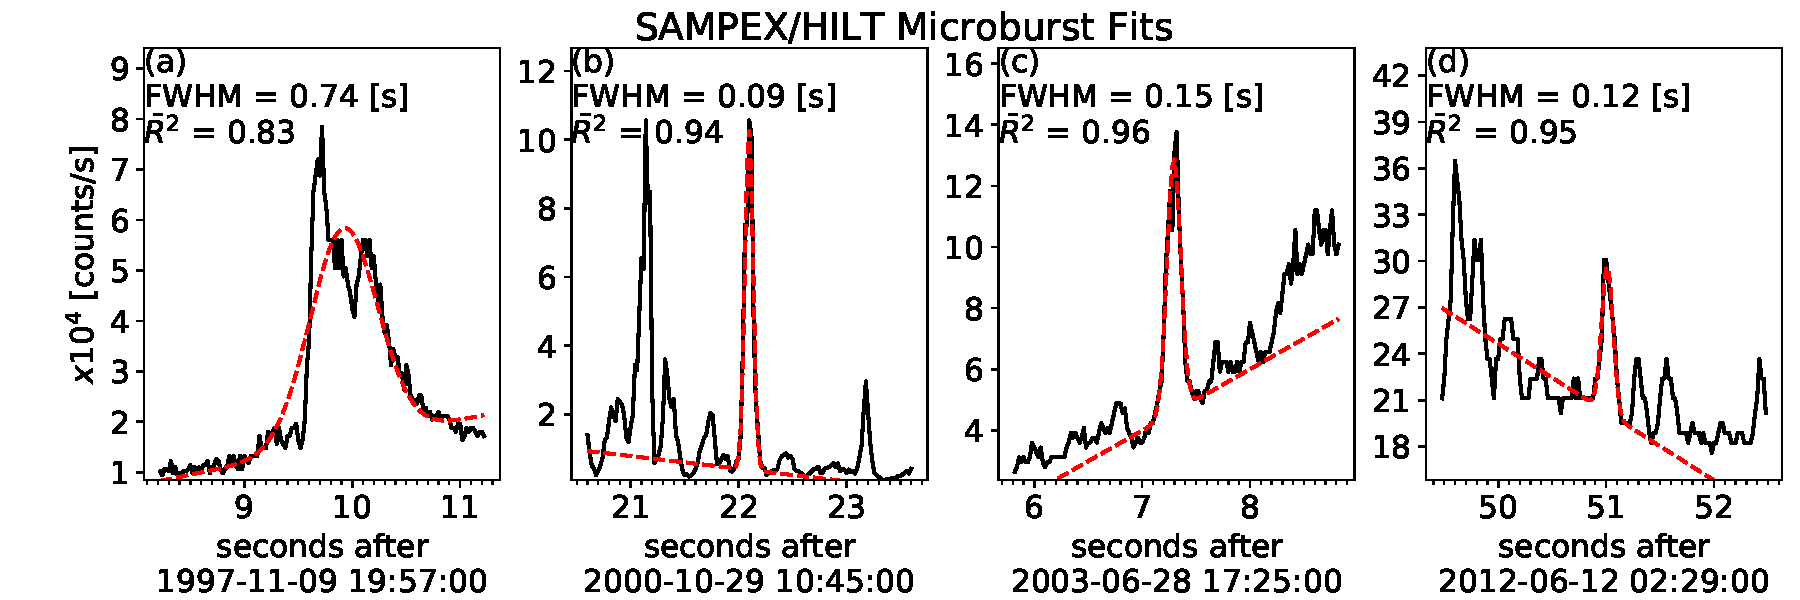
\includegraphics[width=\textwidth]{figures/fig1.pdf}
\caption{Examples of relativistic microbursts are shown by the black curves, and the fits are shown by the dashed red curves. The fit's full width at half maximum (FWHM) and the $\bar{R}^2$ goodness of fit metric is annotated in each panel. Microbursts with $\bar{R}^2 > 0.9$ were used for this study---hence the two-peaked example in panel a was not analyzed. The major time ticks are at every second, while the minor ticks are at every 100 milliseconds.}
\label{fig1}
\end{figure}

\subsection{Microburst Duration Quantification}
Second, we estimated the microburst duration using two methods, detailed below, that yielded similar results: the duration at half of the microburst's topographic prominence and the full width at half maximum (FWHM) from a Gaussian fit.

The topographic prominence is a simple and robust method to estimate the microburst duration previously used to identify curtains, a similar-looking type of precipitation \cite{Shumko2020b}. Using this technique, we define microburst duration to be the duration at half of the microburst's topographic prominence: the height of the microburst relative to the maximum of the two minima on either side of the microburst peak. On each side of the microburst peak, the minima are searched for between the microburst and a higher peak on that side. While the topographic prominence method of estimating microburst durations is simple and robust, a downside is its inability to automatically verify that the estimated duration is of a single microburst and not a superposition of multiple microbursts (Fig. \ref{fig1}a is an example of two superposed microbursts).

To overcome this downside, we fit the microburst time series and used the $R^2$ goodness of fit metric to verify the fit. We assumed a fit model consisting of a Gaussian to model the microburst peak, superposed with a straight line to model the background counts due to drifting electrons at and around the microburst. This model is defined as
\begin{equation}
c(t | A, t_0, \sigma, c_0, c_1) = A e^{-\frac{(t-t_0)^2}{2\sigma^2}} + c_0 + c_1 t
\end{equation} where $A$, $t_0$, and $\sigma$ are the Gaussian amplitude, center time, and standard deviation; $c_0$ and $c_1$ are the linear background count intercept and slope. We determined the number of data points to fit as the maximum of: 4x topographic prominence duration or 500 ms. A challenge to any robust and automated nonlinear regression algorithm is guessing the initial parameters. The initial parameter guesses for the Gaussian are provided by the estimated topographic prominence and duration. The straight line parameter guesses were: $c_0=\mathrm{median(counts)}$ and $c_1=0$. The optimal fit parameters were found using scipy's \url{curve_fit()} function in Python. We defined the microburst duration as the FWHM of the microburst peak, defined by
\begin{equation}
\mathrm{FWHM} = 2\sqrt{2 \ln{2}} \sigma.
\end{equation}

To evaluate the fit, we used the $R^2$ goodness of fit metric. $R^2$ is defined as
\begin{equation}
R^2 = 1 - \frac{SS_{res}}{SS_{mean}} = 1 - \frac{\sum{(c_i-f_i)^2}}{\sum{(c_i-\bar{c})^2}}
\end{equation} where $SS_{res}$ is the sum of the squared residuals between the observed counts $c_i$ and the fit counts $f_i$ for each time step, and likewise $SS_{mean}$ is the sum of the squared residuals between $c_i$ and the mean of the counts, $\bar{c}$.

One interpretation of $R^2$ is fractionally how much better the variance in the data is explained by the model fit, compared to the null hypothesis horizontal line at $\bar{c}$. $R^2$ varies from $1$ for a fit that perfectly describes the data, to $-\infty$ for poor fits (a fit can be much worse than the mean null hypothesis).

To account for overfitting, we used the adjusted $R^2$, $\bar{R}^2$, defined as

\begin{equation}
\bar{R}^2 = 1 - (1-R^2) \frac{n-1}{n-p-1}
\end{equation} where $n$ is the number of data points fit, and $p$ is the number of parameters. Intuitively, $n-1$ is the number of degrees of freedom for the null hypothesis, and $n-p-1$ is the degrees of freedom for the fit model. Fits with $\bar{R}^2 > 0.9$ are considered good and are analyzed. As a check, we compared the microburst duration estimated with the prominence and fit methods. We first chose an agreement criterion between the two methods as a duration within 25\%; together with the $\bar{R}^2 > 0.9$ constraint, $85\%$ of microbursts satisfied these criteria.

Figure \ref{fig1}a shows an example of two superposed microbursts that had a fit $\bar{R}^2 = 0.83$ that were excluded from this study. On other hand, microbursts in Fig. \ref{fig1}b-d had $\bar{R}^2 > 0.9$ and were included in the following analysis. Lastly, Fig. \ref{fig1}c and d demonstrate the necessity of the linear fit to account for the changing background. The linear fit accounts for the non-zero mean background counts and the uneven amplitudes at the edges of the Gaussian. Of the 256,764 detected microbursts, 109,231 have $\bar{R}^2 > 0.9$ and are used for the remainder of this study.

\section{Results}\label{results}
We used the well-fit microbursts to quantify the distribution of microburst duration (FWHM). We then investigated trends in the duration distribution as a function of the Auroral Electrojet index, L-shell and MLT. We begin with the overall microburst distribution.

Figure \ref{fig2}a shows the distribution of all well-fit microbursts. This distribution is strongly peaked with 97 ms median duration. The interquartile range spans about a factor of two in microburst duration, from 66 to 142 ms.

We then investigated the dependence of microburst duration as a function of geomagnetic activity. To be consistent with many prior wave and microburst studies, we use the AE index to quantify the level of geomagnetic disturbance. We adopt the same three AE intensity levels used in prior studies, such as \citeA{Douma2017}, and \citeA{Meredith2020}: $\mathrm{AE} < 100$, $100 < \mathrm{AE} < 300$, and $\mathrm{AE} > 300$, in units of nanotesla (nT). Figure \ref{fig2}b shows the distribution of microburst duration for the three AE categories. The distributions are qualitatively similar, gradually narrowing and shifting to shorter durations with increasing AE. The median microburst duration decreases from 130 ms for $\mathrm{AE} < 100$ to 95 ms for $ \mathrm{AE} > 300$.

\begin{figure}
\noindent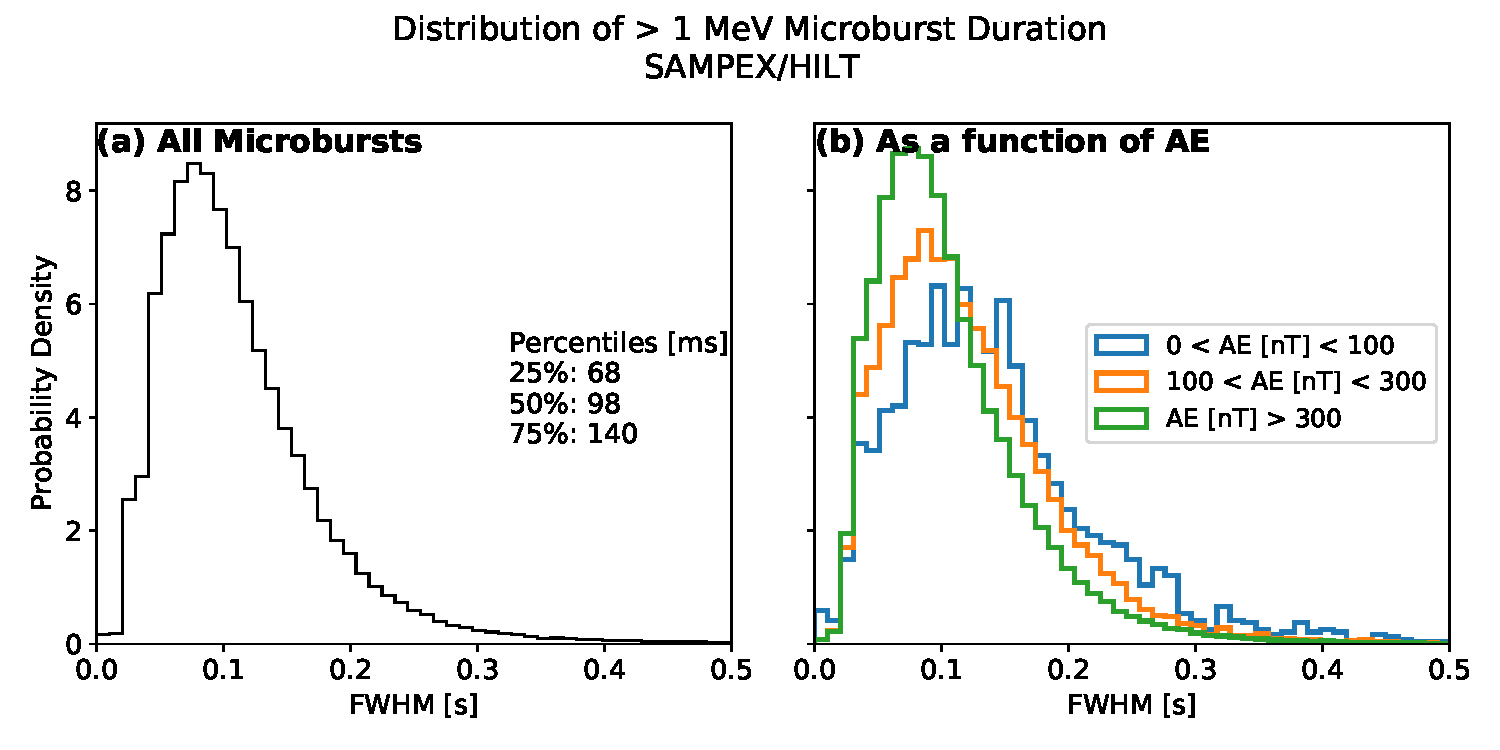
\includegraphics[width=\textwidth]{figures/fig2.pdf}
\caption{Panel a shows the distribution of all microburst full width at full maximum (FWHM). Panel b shows the distribution of all microbursts, categorized by the Auroral Electrojet (AE) index into three bins: $\mathrm{AE} < 100$, $100 < \mathrm{AE} < 300$, and $\mathrm{AE} > 300$, in units of nT. The median microburst duration is 130 ms for the $\mathrm{AE} < 100$ ($2.4\times 10^{3}$ microbursts), 111 ms for the $100 < \mathrm{AE} < 300$ ($1.8\times 10^{4}$ microbursts), and 95 ms for the $ \mathrm{AE} > 300$ ($9.3\times 10^{4}$ microbursts) bins.}
\label{fig2}
\end{figure}

\DIFdelbegin \DIFdel{Lastly, Figs. }\DIFdelend \DIFaddbegin \DIFadd{Figures }\DIFaddend \ref{fig3} and \ref{fig4} show the microburst duration as a function of L and MLT. Figure \ref{fig3}a shows the median microburst distribution, while Figure \ref{fig4} shows the marginalized distributions as a function of L or MLT. The median microburst duration trend in Fig. \ref{fig3}a roughly doubles \DIFaddbegin \DIFadd{in MLT}\DIFaddend : from 80 ms at midnight to 160 ms at noon\DIFdelbegin \DIFdel{MLT}\DIFdelend . In L-shell, the median microburst duration slightly increases with L-shell, most apparent near midnight MLT.

To disentangle the L and MLT distributions, Fig. \ref{fig4} shows the marginalized distributions; MLT was marginalized out (summed over) in Fig. \ref{fig4}a and L-shell was marginalized out in Fig. \ref{fig4}b. Figure \ref{fig4}a shows a \DIFdelbegin \DIFdel{slight }\DIFdelend \DIFaddbegin \DIFadd{gradual }\DIFaddend broadening and shifting of the microburst duration \DIFdelbegin \DIFdel{. The median duration}\DIFdelend \DIFaddbegin \DIFadd{in L: the median duration, shown by the solid white line, }\DIFaddend increases from 85 \DIFdelbegin \DIFdel{to 106 ms for }\DIFdelend \DIFaddbegin \DIFadd{ms at }\DIFaddend L=4\DIFdelbegin \DIFdel{to }\DIFdelend \DIFaddbegin \DIFadd{, to 106 ms at }\DIFaddend L=5.5\DIFdelbegin \DIFdel{and then slightly decreases at higher L-shells. In contrast , }\DIFdelend \DIFaddbegin \DIFadd{. This trend is in stark contrast to }\DIFaddend Fig. \ref{fig4}b \DIFdelbegin \DIFdel{, }\DIFdelend that clearly shows the microburst duration \DIFdelbegin \DIFdel{increase from midnight to }\DIFdelend \DIFaddbegin \DIFadd{roughly double from 75 ms near midnight to 140 ms near }\DIFaddend noon MLT.

\begin{figure}
\noindent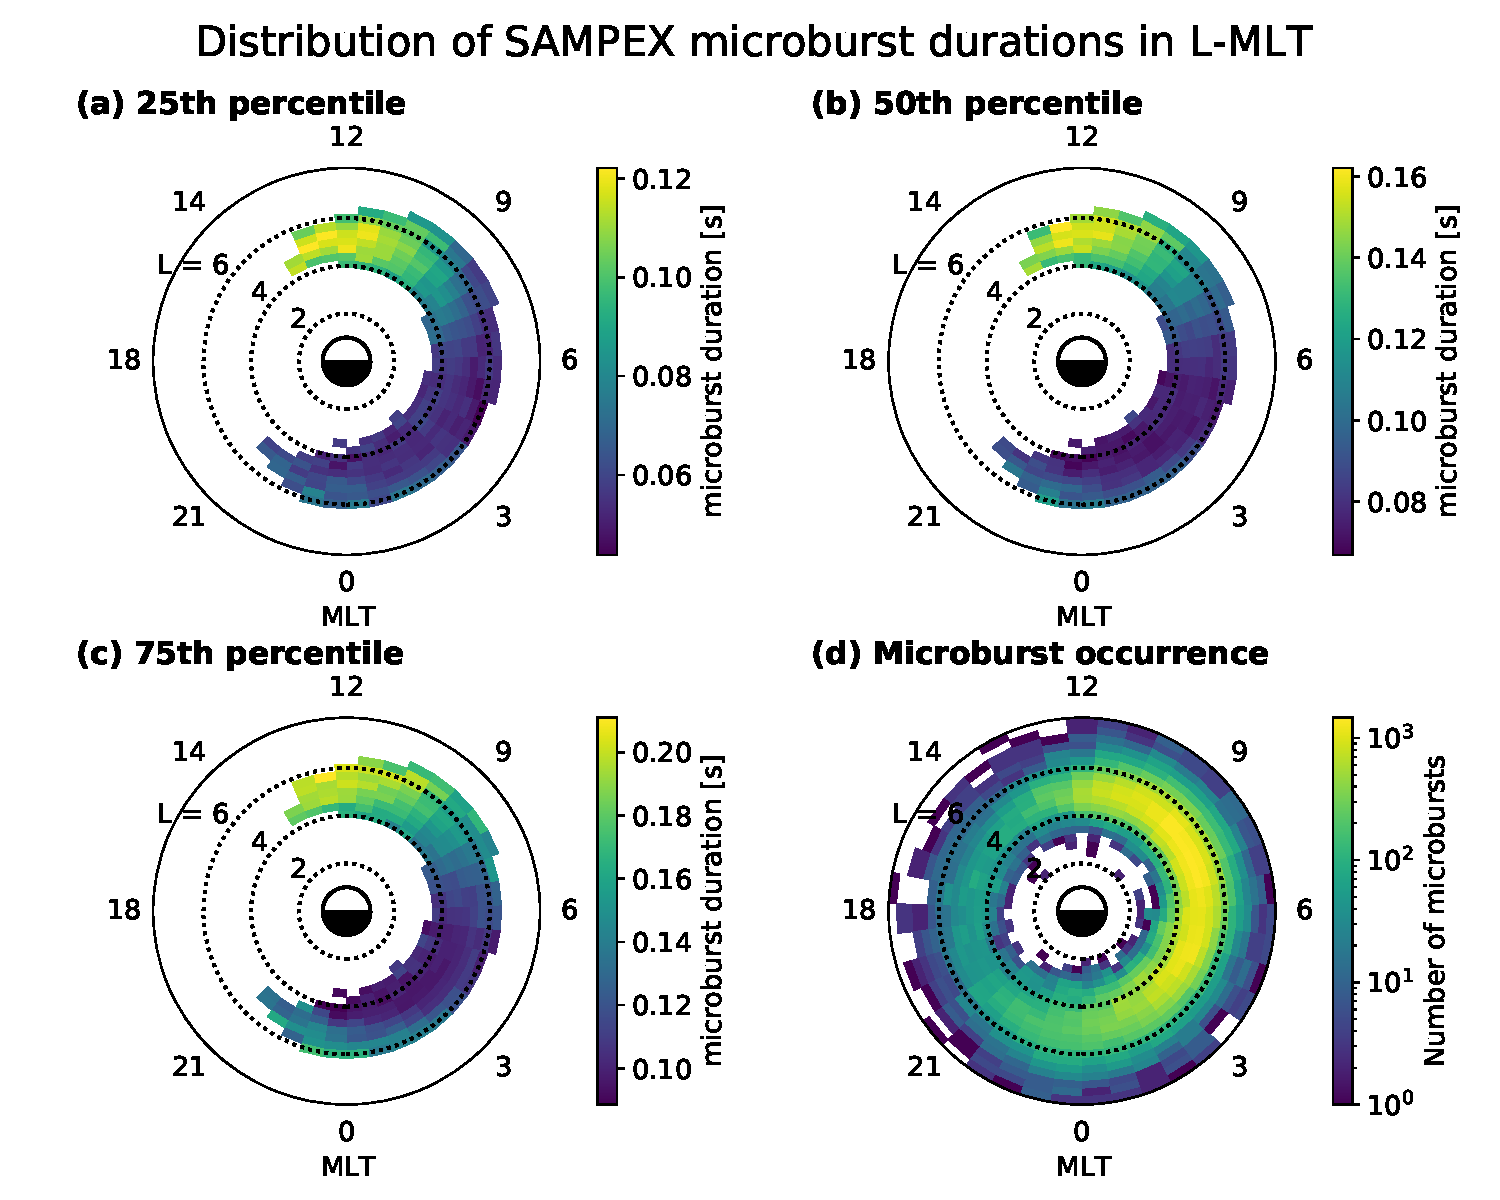
\includegraphics[width=\textwidth]{figures/fig3.pdf}
\caption{Panel a shows the joint distribution of the median microburst duration (FWHM) as a function of L-Shell and MLT. The white bins in panel a have less than 100 microbursts and are statistically insufficient. Panel b shows the distribution of the number of microbursts, with the white bins containing 0 microbursts.}
\label{fig3}
\end{figure}

\begin{figure}
\noindent\DIFdelbeginFL %DIFDELCMD < 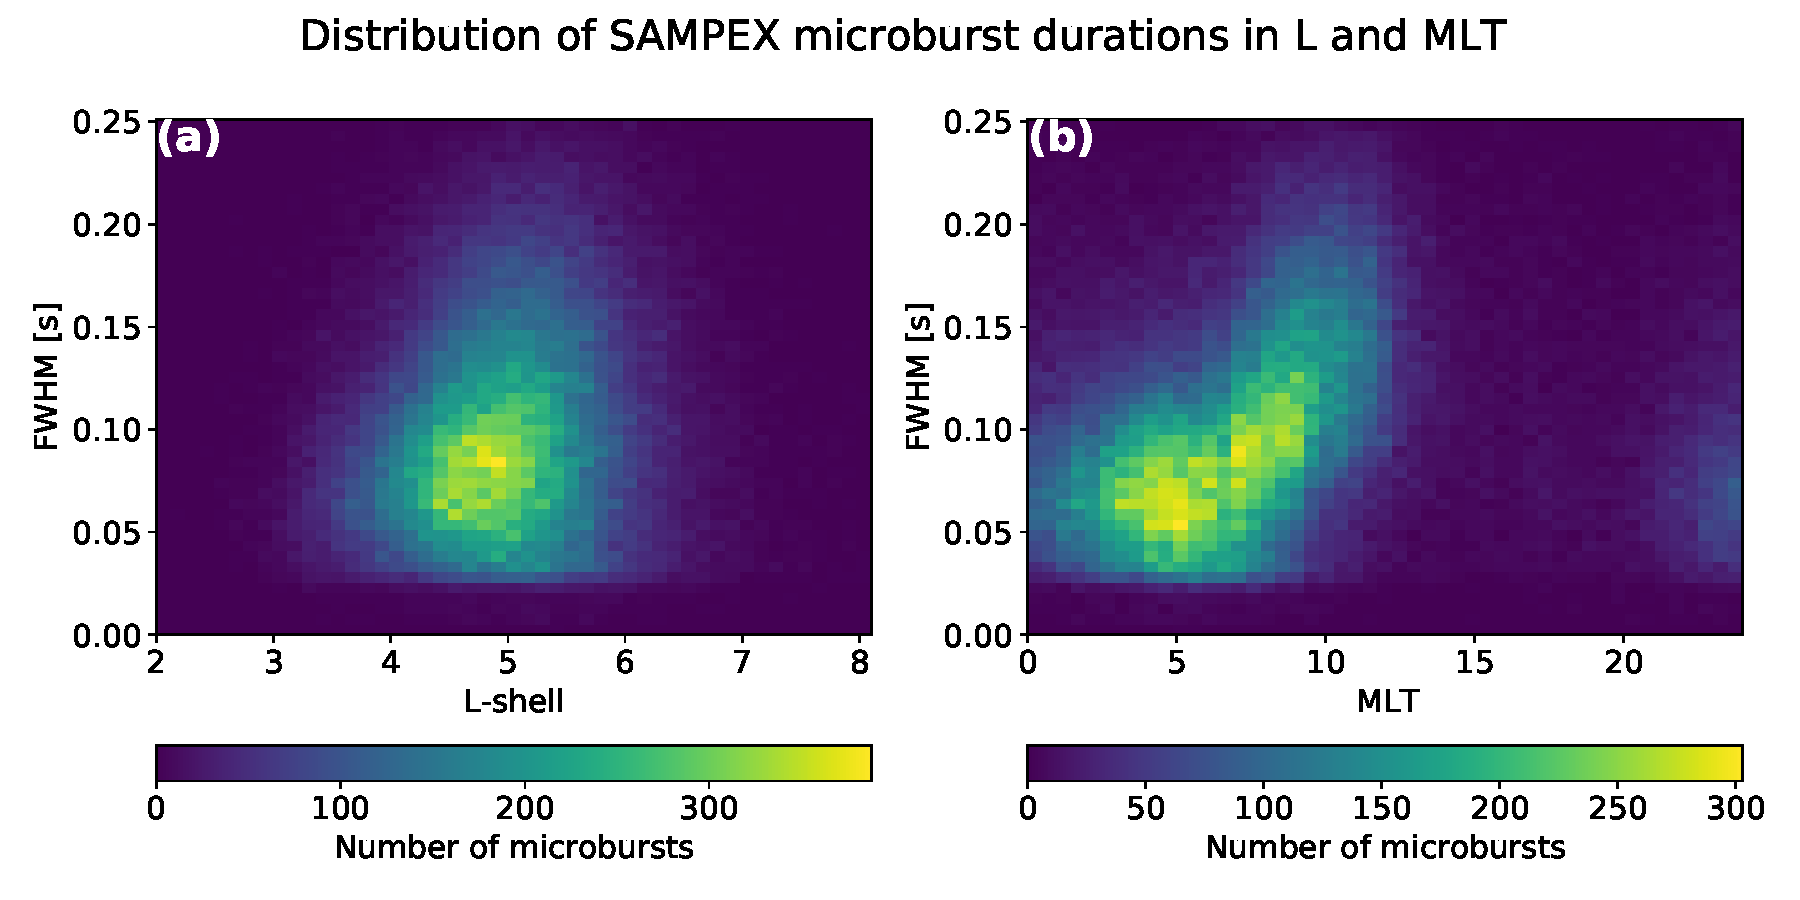
\includegraphics[width=\textwidth]{figures/fig4.pdf}
%DIFDELCMD < %%%
\DIFdelendFL \DIFaddbeginFL 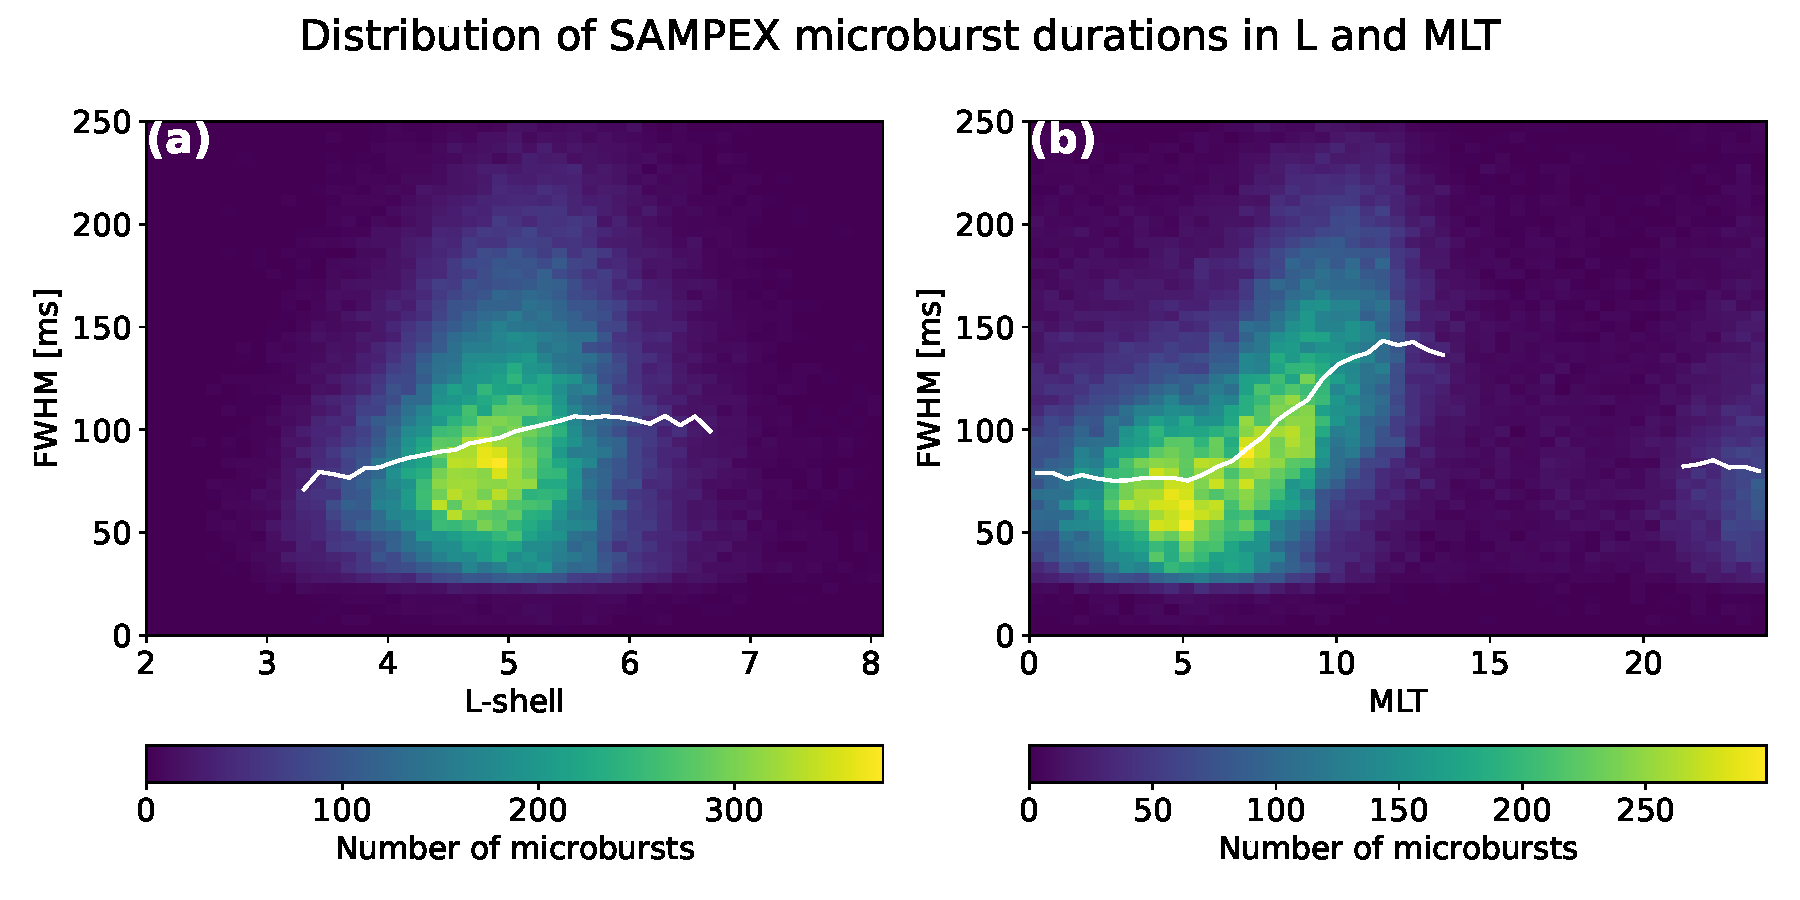
\includegraphics[width=\textwidth]{figures/fig4_v7.pdf}
\DIFaddendFL \caption{The marginalized distributions of the number of microbursts as a function of microburst duration (FWHM) and \DIFdelbeginFL \DIFdelFL{L shell }\DIFdelendFL \DIFaddbeginFL \DIFaddFL{L-shell }\DIFaddendFL in panel a, and MLT in panel b. \DIFaddbeginFL \DIFaddFL{The white lines show the median duration in each L-shell and MLT bins.}\DIFaddendFL }
\label{fig4}
\end{figure}

\section{Discussion and Conclusions}\label{discussion}

We found that $>1$ MeV microbursts have a duration distribution peaked at $\approx 100$ ms, with 50\% of microburst durations between $66-142$ ms. Microburst durations slightly \DIFdelbegin \DIFdel{shrink }\DIFdelend \DIFaddbegin \DIFadd{decrease }\DIFaddend with increasing AE index. We found a significant trend in MLT---the median microburst duration doubles from 80 to 160 ms between midnight and noon MLT. However, before we put these results in the bigger context, we first need to understand how our choice of microburst detection algorithm can lead to reduced sensitivity to microbursts that are longer than $\approx 200$ ms.

Recall from Section \ref{microburst_id} that $A$ is the running average counts, centered on the foreground counts $N$, and the burst parameter, $n_\sigma \sim N - A$. Now consider the following hypothesized scenario. Given a microburst with a 500 ms duration and the burst parameter centered on the peak, $A_{500}$ completely overlaps with the microburst and is therefore the mean microburst counts. Then, $n_\sigma$ is proportional to the difference between the mean and the maximum microburst amplitude. However, if we use $A_{1000}$, it no longer overlaps with just the microburst, but rather the microburst and the lower surrounding background. The resulting $A_{1000}$ is lower than $A_{500}$---thus the $A_{1000}$ burst parameter is more sensitive to the microburst.

To test this possible bias, we ran the detection algorithm with three background values: $A_{500}$, $A_{1000}$, and $A_{2000}$ and compared the resulting median distributions. The maximum discrepancy in the median microburst duration, using the three resulting data sets, was 20 ms---one HILT time sample. This is a 20\% relative discrepancy. Consequently, considering this bias and the distribution in Fig. \ref{fig2}a, the evidence supports that the majority of $>1$ MeV microbursts have a true duration around 100 ms and the $A_{500}$ is adequate to identify them. With more confidence in the detection algorithm, we now discuss the global distribution of microburst durations.

The microburst duration trend in L-shell is subtle\DIFdelbegin \DIFdel{: }\DIFdelend \DIFaddbegin \DIFadd{. Figure \ref{fig4}a shows that }\DIFaddend the median microburst duration increases from 85 to 106 ms between L=4 and \DIFaddbegin \DIFadd{L=}\DIFaddend 5.5 and then decreases to 90 ms at L=7. \DIFdelbegin \DIFdel{This subtle trend is most evident in Fig. \ref{fig4}a. }\DIFdelend In contrast, the duration trend in MLT is significant. Figure \ref{fig4}b shows that the median microburst duration doubles from \DIFdelbegin \DIFdel{80 to 160 }\DIFdelend \DIFaddbegin \DIFadd{75 to 140 }\DIFaddend ms between midnight and noon MLT. Now we will focus on the MLT trend and look for a possible explanation.

As mention in the introduction, chorus rising tone elements are widely believed to scatter microburst electrons \cite<e.g.>{Breneman2017, Saito2012, Miyoshi2020}. Thus, we will compare the microburst duration and chorus trends in local time. Recent studies by \citeA{Teng2017} and \citeA{Shue2019} quantified the properties of equatorial lower band (0.1-0.5 x electron gyrofrequency) chorus rising tone elements. Both studies found that the rising tone element duration distribution peaks at $\approx 250$ ms around midnight, and broadening and shifting to $\approx 500$ ms at noon. The previous chorus duration results and our microburst duration results both found that their durations roughly double from midnight to noon MLT. However, the chorus durations are about 3-4x longer than the microbursts. This scaling is consistent with \citeA{Miyoshi2020} who predicted a similar difference in duration between chorus rising tone element and relativistic microburst durations.

As a function of AE, the median microburst duration decreases from 130 ms, for $AE < 100$ nT, to 95 ms for $AE > 300$ nT. The chorus rising tone duration trend, quantified by \citeA{Teng2017}, is similar: it is broad and peaks at $\approx 500$ ms for $AE < 100$ nT, then narrows and shifts to $\approx 250$ ms for $AE > 300$ nT. While both become shorter with increased AE, the change in microburst duration is relatively smaller than the change in chorus duration.

Numerous test particle simulations have been performed to study the relationship between chorus rising tone elements and microbursts. \citeA{Chen2020} found that medium energy ($\approx 50-300$ keV) microburst duration is controlled by the rising tone element bandwidth. Moreover, higher energy microburst duration is controlled by the wave's lower frequency and the absolute value of the upper magnetic latitude of propagation. Their results are in qualitative agreement with the cyclotron resonance condition described in \citeA{Lorentzen2001a}, and the simulated electron \DIFdelbegin \DIFdel{time of flight }\DIFdelend \DIFaddbegin \DIFadd{time-of-flight }\DIFaddend described by \citeA{Saito2012}.

While different model parameters may change what wave properties are theoretically responsible for scattering $>1$ MeV microburst electrons, it is worth noting that Figs. 4 and 5 in \citeA{Shue2019} do not show a clear shift in chorus bandwidth between midnight and noon MLT. Care must be taken when comparing our results to theory: HILT measured multi-energy microburst electrons above 1 MeV, and microbursts at each energy can have different drivers and durations, as simulated by \citeA{Chen2020} and \citeA{Miyoshi2020}. Nevertheless, theory does not conclusively predict what chorus wave properties control the $> 1$ MeV microburst duration, but the chorus rising tone duration trend in MLT is worth further consideration. 

Lastly, high latitude chorus waves, \DIFdelbegin \DIFdel{found }\DIFdelend \DIFaddbegin \DIFadd{observed }\DIFaddend at $|\lambda| \approx 10^\circ-25^\circ$ magnetic \DIFdelbegin \DIFdel{latitude off of the equator}\DIFdelend \DIFaddbegin \DIFadd{latitudes}\DIFaddend , can also play at important role at scattering microburst electrons \cite{Lorentzen2001a}. \DIFdelbegin \DIFdel{\mbox{%DIFAUXCMD
\citeA{Li2009a} }\hspace{0pt}%DIFAUXCMD
found that the majority of high latitude chorus waves are constrained to 6-12 MLT . Thus, it is tempting to conclude that the microburst duration trend in MLT could be attributed to some difference in how low and high latitude chorus waves scatter MeV electrons. However, because low latitude chorus waves are also observed at 0-12 MLT, the resulting microburst duration distribution would reflect the }\DIFdelend \DIFaddbegin \DIFadd{Figure 9 in \mbox{%DIFAUXCMD
\citeA{Agapitov2018b} }\hspace{0pt}%DIFAUXCMD
shows the }\DIFaddend chorus \DIFdelbegin \DIFdel{wave superposition in }\DIFdelend \DIFaddbegin \DIFadd{occurrence and root-mean-square wave amplitude as a function of $\lambda$ and wave normal angle in three MLT bins. In two of their MLT bins that are relevant here: 21-3 and 4-12 hours, }\DIFaddend the \DIFdelbegin \DIFdel{6-12 MLT region. If low and high latitude chorus waves scattered microbursts with different durations, Fig. \ref{fig4}b would show the microburst durations broaden or bifurcate from midnight to noon MLT. Because Fig. \ref{fig4}b shows the entire microburst duration distributionshifting to longer durations, high vs low latitude chorus waves are an unlikely explanation for the microburst duration trend in MLT}\DIFdelend \DIFaddbegin \DIFadd{occurrence probability is largely independent of $|\lambda|$. But this is not the case for the chorus wave amplitude; it is mostly confined to $|\lambda| < 7^\circ$ in 21-3 MLT and $|\lambda| > 5^\circ$ in 4-12 MLT. The chorus amplitude-MLT-$|\lambda|$ distribution, together with the time-of-flight effect, is another persuasive mechanism for differing microburst durations that is also worth further consideration}\DIFaddend . 

In summary, we found that the relativistic microburst duration distribution is peaked at 100 ms, with 75\% of microbursts narrower than 140 ms. We discovered a strong trend in microburst duration as a function of MLT---the median microburst duration roughly doubling from \DIFdelbegin \DIFdel{80 ms at }\DIFdelend \DIFaddbegin \DIFadd{75 ms near }\DIFaddend midnight, to \DIFdelbegin \DIFdel{160 ms at }\DIFdelend \DIFaddbegin \DIFadd{140 ms near }\DIFaddend noon. Prior work also shows that chorus rising tone element durations double in MLT \DIFaddbegin \DIFadd{\mbox{%DIFAUXCMD
\cite{Shue2019,Teng2017}}\hspace{0pt}%DIFAUXCMD
}\DIFaddend . At a given local time, the rising tone element duration \DIFaddbegin \DIFadd{is }\DIFaddend 3-4 times longer. These results indicate a likely relationship between durations of chorus rising tone elements and microbursts, and we encourage future modeling work to explore this relationship.


%%%%%%%%%%%%%%%%%%%%%%%%%%%%%%%%
%% Optional Appendix goes here
%
% The \appendix command resets counters and redefines section heads
%
% After typing \appendix
%
%\section{Here Is Appendix Title}
% will show
% A: Here Is Appendix Title
%
%\appendix
%\section{Here is a sample appendix}

\acknowledgments
We are thankful for the engineers and scientists who made the SAMPEX mission possible. M. Shumko acknowledges the support provided by the NASA Postdoctoral Program at the NASA’s Goddard Space Flight Center, administered by Universities Space Research Association under contract with NASA; L.W.Blum acknowledges the Heliophysics Innovation Fund program at NASA’s Goddard Space Flight Center; and A.B. Crew acknowledges funding provided by the National Science Foundation, award 1602607. The SAMPEX HILT and attitude data are \DIFdelbegin \DIFdel{located at }\DIFdelend \DIFaddbegin \DIFadd{only available at the following FTP link }\DIFaddend \url{http://www.srl.caltech.edu/sampex/DataCenter/data.html}\DIFaddbegin \DIFadd{, }\DIFaddend and the minute cadence Auroral Electrojet data is \DIFdelbegin \DIFdel{located }\DIFdelend \DIFaddbegin \DIFadd{available }\DIFaddend at \url{ftp://ftp.ngdc.noaa.gov/STP/GEOMAGNETIC_DATA/INDICES/AURORAL_ELECTROJET/ONE_MINUTE/}.
This analysis software is available at: \url{https://github.com/mshumko/sampex_microburst_widths}, and is archived on Zenodo \DIFdelbegin %DIFDELCMD < \url{https://doi.org/10.5281/zenodo.4687987}
%DIFDELCMD < %%%
\DIFdelend \DIFaddbegin \url{https://doi.org/10.5281/zenodo.4961209}
\DIFaddend 


%% ------------------------------------------------------------------------ %%
%% References and Citations

%%%%%%%%%%%%%%%%%%%%%%%%%%%%%%%%%%%%%%%%%%%%%%%
%
% \bibliography{<name of your .bib file>} don't specify the file extension
%
% don't specify bibliographystyle
%%%%%%%%%%%%%%%%%%%%%%%%%%%%%%%%%%%%%%%%%%%%%%%

\bibliography{refs.bib}



%Reference citation instructions and examples:
%
% Please use ONLY \cite and \citeA for reference citations.
% \cite for parenthetical references
% ...as shown in recent studies (Simpson et al., 2019)
% \citeA for in-text citations
% ...Simpson et al. (2019) have shown...
%
%
%...as shown by \citeA{jskilby}.
%...as shown by \citeA{lewin76}, \citeA{carson86}, \citeA{bartoldy02}, and \citeA{rinaldi03}.
%...has been shown \cite{jskilbye}.
%...has been shown \cite{lewin76,carson86,bartoldy02,rinaldi03}.
%... \cite <i.e.>[]{lewin76,carson86,bartoldy02,rinaldi03}.
%...has been shown by \cite <e.g.,>[and others]{lewin76}.
%
% apacite uses < > for prenotes and [ ] for postnotes
% DO NOT use other cite commands (e.g., \citet, \citep, \citeyear, \nocite, \citealp, etc.).
%

\end{document}